\documentclass[coursework]{SCWorks}
% Тип обучения (одно из значений):
%    bachelor   - бакалавриат (по умолчанию)
%    spec       - специальность
%    master     - магистратура
% Форма обучения (одно из значений):
%    och        - очное (по умолчанию)
%    zaoch      - заочное
% Тип работы (одно из значений):
%    coursework - курсовая работа (по умолчанию)
%    referat    - реферат
%  * otchet     - универсальный отчет
%  * nirjournal - журнал НИР
%  * digital    - итоговая работа для цифровой кафдры
%    diploma    - дипломная работа
%    pract      - отчет о научно-исследовательской работе
%    autoref    - автореферат выпускной работы
%    assignment - задание на выпускную квалификационную работу
%    review     - отзыв руководителя
%    critique   - рецензия на выпускную работу
% Включение шрифта
%    times      - включение шрифта Times New Roman (если установлен)
%                 по умолчанию выключен
\usepackage{preamble}

\begin{document}

% Кафедра (в родительном падеже)
\chair{математической кибернетики и компьютерных наук}

% Тема работы
\title{ЛЕКСИЧЕСКИЙ И СИНТАКСИЧЕСКИЙ АНАЛИЗ ВЫРАЖЕНИЙ}

% Курс
\course{1}

% Группа
\group{151}

% Факультет (в родительном падеже) (по умолчанию "факультета КНиИТ")
% \department{факультета КНиИТ}

% Специальность/направление код - наименование
% \napravlenie{02.03.02 "--- Фундаментальная информатика и информационные технологии}
% \napravlenie{02.03.01 "--- Математическое обеспечение и администрирование информационных систем}
% \napravlenie{09.03.01 "--- Информатика и вычислительная техника}
\napravlenie{09.03.04 "--- Программная инженерия}
% \napravlenie{10.05.01 "--- Компьютерная безопасность}

% Для студентки. Для работы студента следующая команда не нужна.
% \studenttitle{Студентки}

% Фамилия, имя, отчество в родительном падеже
\author{Голышева Юрия Олеговича}

% Заведующий кафедрой 
\chtitle{доцент, к.\,ф.-м.\,н.}
\chname{С.\,В.\,Миронов}

% Руководитель ДПП ПП для цифровой кафедры (перекрывает заведующего кафедры)
% \chpretitle{
%     заведующий кафедрой математических основ информатики и олимпиадного\\
%     программирования на базе МАОУ <<Ф"=Т лицей №1>>
% }
% \chtitle{г. Саратов, к.\,ф.-м.\,н., доцент}
% \chname{Кондратова\, Ю.\,Н.}

% Научный руководитель (для реферата преподаватель проверяющий работу)
\satitle{доцент, к.\,ф.-м.\,н.} %должность, степень, звание
\saname{Г.\,Г.\,Наркайтис}

% Руководитель практики от организации (руководитель для цифровой кафедры)
\patitle{доцент, к.\,ф.-м.\,н.}
\paname{С.\,В.\,Миронов}

% Руководитель НИР
\nirtitle{доцент, к.\,п.\,н.} % степень, звание
\nirname{В.\,А.\,Векслер}

% Семестр (только для практики, для остальных типов работ не используется)
\term{2}

% Наименование практики (только для практики, для остальных типов работ не
% используется)
\practtype{учебная}

% Продолжительность практики (количество недель) (только для практики, для
% остальных типов работ не используется)
\duration{2}

% Даты начала и окончания практики (только для практики, для остальных типов
% работ не используется)
\practStart{01.07.2022}
\practFinish{13.01.2023}

% Год выполнения отчета
\date{2023}

\maketitle

% Включение нумерации рисунков, формул и таблиц по разделам (по умолчанию -
% нумерация сквозная) (допускается оба вида нумерации)
%\secNumbering

\tableofcontents

% Раздел "Обозначения и сокращения". Может отсутствовать в работе
% \abbreviations
% \begin{description}
%     \item ... "--- ...
%     \item ... "--- ...
% \end{description}

% Раздел "Определения". Может отсутствовать в работе
% \definitions

% Раздел "Определения, обозначения и сокращения". Может отсутствовать в работе.
% Если присутствует, то заменяет собой разделы "Обозначения и сокращения" и
% "Определения"
% \defabbr

\intro
Лексические и синтаксические анализаторы как предмет научного исследования появились в 1950-х годах XX века. Бурный рост интереса был обусловлен в том числе необходимостью создания интерпретаторов и компиляторов для трансляции языков высокого уровня в другие языки или напрямую в машинный код.

Несмотря на то, что сейчас эта область является хорошо изученной, она все еще актуальна и находит свои применения при создании статических и динамических компиляторов, трансляции одних языков программирования в другие, обработке SQL-запросов и некоторых других классов задач\cite{1,2}. Необходимость быстрого анализа при этом очевидна.

Целью данной работы является изучение работы лексических и синтаксических анализаторов и повышение эффективности анализа за счет различных оптимизаций работы с оперативной памятью.

В ходе написания работы должны быть решены следующие задачи:
\begin{enumerate}
    \itemИзучение понятий лексического и синтаксического анализа.
    \itemАнализ технических особенностей реализации лексических и синтаксических анализаторов и изучение работы генераторов лексического и синтаксического анализа на примере Flex и GNU Bison.
    \itemСоздание лексического и синтаксического анализатора для анализа математического выражения.
    \itemИзучение понятия абстрактного синтаксического дерева.
    \itemСоздание нескольких реализаций абстрактного синтаксического дерева для построенной грамматики и сравнение эффективности их работы.
\end{enumerate}
% После введения — серии \section, \subsection и т.д.
\section{Управление памятью на основе регионов}
\subsection{Мотивировка}
Текущая реализация абстрактного синтаксического дерева имеет следующие недостатки:
\begin{enumerate}
    \itemВыделение памяти стандартным методом может значительно фрагментировать оперативную память, затрудняя доступ к ней.
    \itemЛюбое выделение и удаление памяти требует вмешательства системных вызовов, что может стать причиной дополнительных издержек во время работы программы.
    \itemПрограммист не имеет возможности ручного управления выделяемой им памятью.
\end{enumerate}

Избавиться от этих недостатков можно используя различные оптимизации. В рамках этой работы воспользуемся управлением памятью на основе, так называемых, регионов (арен, зон)\cite{11}.

Под регионом далее будем понимать непрерывную область памяти, содержащую внутри себя объекты. При запуске программы выделим регион некоторого размера, при необходимости увеличивая его размер в некоторое постоянное число раз.

Этот подход имеет следующие преимущества:
\begin{enumerate}
    \itemЭлементы располагаются последовательно, в связи с чем минимизируется фрагментация и упрощается доступ к объектам.
    \itemВыделение и освобождение памяти выполняется с минимальными издержками.
    \itemПрограммисту предоставляется большая свобода для управления выделенной памятью.
\end{enumerate}
\subsection{Построение}
Формально определим требования к системе:
\begin{enumerate}
    \itemРегион должен представлять из себя некоторый непрерывный участок размера $n$ байт (в начальный момент времени размер равен некоторой начальной величине $n_0$).
    \itemПри обращении к региону он должен предоставить $k$ байт памяти и вернуть некоторый идентификатор этого участка для последующего обращения.
    \itemПри заполнении региона должна быть возможность увеличить объем доступной памяти в некоторое число раз, которое далее будем называть коэффициентом увеличения.
    \itemДолжна быть доступна возможность эффективного освобождения всей выделенной регионом памяти.
\end{enumerate}

Единственной сложной операцией над регионом является его увеличение. Так как выделение нового участка потенциально может сопровождаться изменением адресов объектов, то необходимо организовать доступ к ним независимо от первоначального адреса. Для этого для каждого объекта будем получать доступ к нему через некоторый индекс.

Кроме того, коэффициент увеличения должен быть выбран таким образом, чтобы был соблюден баланс между оптимальным объемом выделенной памяти и частотой системных вызовов.

\subsection{Определение структуры}
Определим нашу структуру следующим образом:
\begin{minted}{cpp} 
typedef struct arena {
    // Указатель на начало региона
    struct node* arena;
    // Размер региона
    unsigned int size;
    // Объем выделенной регионом памяти
    unsigned int allocated;
} arena;
\end{minted}

\subsection{Инициализация}
Теперь определим функцию  \texttt{arena\_construct}, выполняющую начальную инициализацию состояния региона:
\begin{minted}{cpp} 
int arena_construct (arena* arena) {
    // Начальный размер региона равен некоторой постоянной, равной DEFAULT_ARENA_SIZE
    arena->size = DEFAULT_ARENA_SIZE;
    arena->allocated = 0;
    // Выделим необходимое число памяти
    arena->arena = malloc(sizeof(node) * DEFAULT_ARENA_SIZE);
    // Если выделение прошло неудачно - вернем в качестве кода ошибки отличное от 0 значение.
    if (arena->arena == NULL) {
        return (!0);
    }
    return 0;
}
\end{minted}
\subsection{Выделение памяти}
    После выделения некоторого объема памяти возможно обращение к ней. Определим это обращение с помощью функции \texttt{arena\_allocate}:
\begin{minted}{cpp} 
int arena_allocate (arena* arena, unsigned int count) {
    // Если места в регионе недостаточно
    if (arena->allocated + count >= arena->size) {
        // Определим новый размер региона
        unsigned int newSize = MULTIPLY_FACTOR * arena->size;
        // Выделим регион большего размера и освободим ранее занятую память
        node* newArena = realloc(arena->arena, 
            newSize * sizeof(node));
        if (NULL == newArena) {
            return -1;
        }
        arena->arena = newArena;
        arena->size = newSize;
    }
    // В качестве результата вернем индекс первого свободного участка региона
    unsigned int result = arena->allocated;
    // Сместим индекс на объем выделенной памяти
    arena->allocated += count;
    // Вернем результат
    return result;
}
\end{minted}
Отметим, что наиболее часто значением \texttt{MULTIPLY\_FACTOR} оказывается числа
1.5 и 2. Это позволяет достичь амортизационно константного времени выполнения операции выделения памяти\cite{12}.
\subsection{Освобождение выделенной памяти}
Наконец, реализуем освобождение выделенной региону памяти с помощью функции \texttt{arena\_free}
\begin{minted}{cpp} 
void arena_free (arena* arena) {
    if (arena->arena != NULL)
        free(arena->arena);
    arena->arena = NULL;
}
\end{minted}
\subsection{Модификация абстрактного синтаксического дерева}
Осталось изменить исходный код программы, чтобы обеспечить выделение памяти с помощью полученной нами структуры данных.

Для этого воспользуемся директивой \texttt{\%param} и заявим в качестве параметра переменную типа \texttt{arena*}. В функциях \texttt{eval}, \texttt{newnum}, \texttt{newast} внесем изменения, чтобы обеспечить выделение памятью с помощью написанных ранее функций.

С полным кодом программы можно ознакомиться в приложении \ref{app:А}.

\subsection{Сборка проекта}
Теперь проект можно собрать, незначительно изменив \texttt{Makefile}:
\begin{minted}{cpp} 
calc.out: calc.l calc.y arena_ast.h
    bison -d calc.y
    flex calc.l
    cc -o $@ calc.tab.c lex.yy.c arena_ast.c arena.c
\end{minted}
и запустить. Результат работы программы представлен на рис. \ref{fig:1}

\begin{figure}[h]

\centering

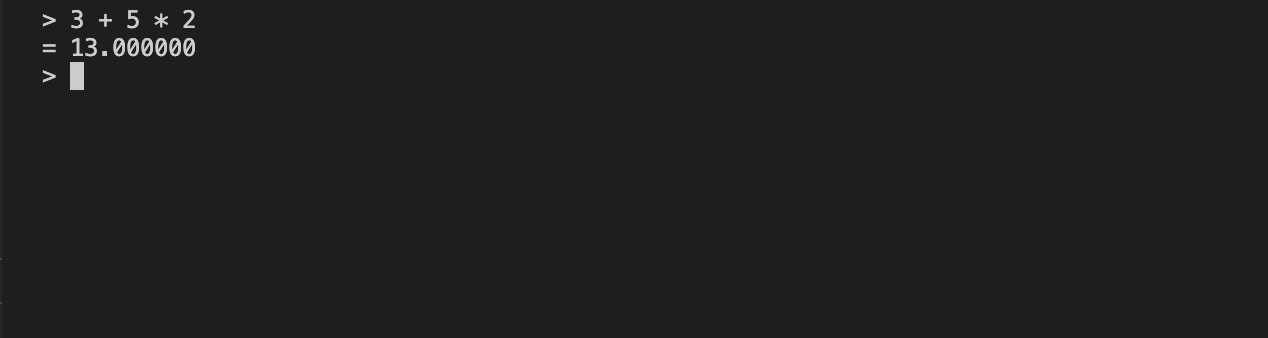
\includegraphics[scale=0.5]{naivetest.png}

\caption{Демонстрация работы программы}

\label{fig:1}

\end{figure}

\section{Сравнение полученных реализаций}
Проведем анализ производительности полученных версий анализатора. В качестве данных для тестирования возьмем выражения вида $\underbrace{2+2+2\dots+2}_{n}$ для  $n$ =  1\dots100 с шагом 1. Для вычисления времени выполнения воспользуемся библиотекой \texttt{time} Python 3.9.5. Автоматизацию обеспечим с помощью
библиотеки \texttt{subprocess}. Получим следующий код:
\begin{minted}{python} 
import subprocess as sb
import time
import sys
def run(args):
    return sb.run(args,
        capture_output=True, ).stdout.decode().strip()

def main():
    if (len(sys.argv) < 6):
    print("Invalid arguments")
    return
    exe_path = sys.argv[1]
    out_path = sys.argv[2]
    right_bound = int(sys.argv[3])
    step = int(sys.argv[4])
    iter = sys.argv[5]

    f = open(out_path, "w")
    f.write(f"{exe_path}\n")
    f.close()
    for expr_len in range(1, right_bound, step):
        test_string = "+".join(['2'] * expr_len)
        args = [exe_path, test_string, iter]
        t = time.monotonic()
        run(args)
        end_t = time.monotonic()
        f = open(out_path, "a")
        f.write(f"{expr_len} {(end_t - t) / (int(iter))}\n")
        f.close()
        print(f" Step {expr_len} finished")

if __name__ == "__main__" :
    main()
\end{minted}

Кроме того, отметим, что в ранее написанные программы были внесены некоторые изменения для проведения эксперимента. Ознакомиться с ними можно в приложении \ref{app:А}.

Ознакомиться с полным исходным кодом программы, осуществляющей исследование производительности можно в приложении \ref{app:Б}.

Для большей наглядности графики интерполированы полиномом с помощью функции \texttt{polyfit} библиотеки \texttt{numpy}.

Ознакомиться с полным исходным кодом программы, осуществляющей анализ полученных результатов можно в приложении \ref{app:В}.

Результаты исследования изображены на рис. \ref{fig:2}:

\begin{figure}[h]

\centering

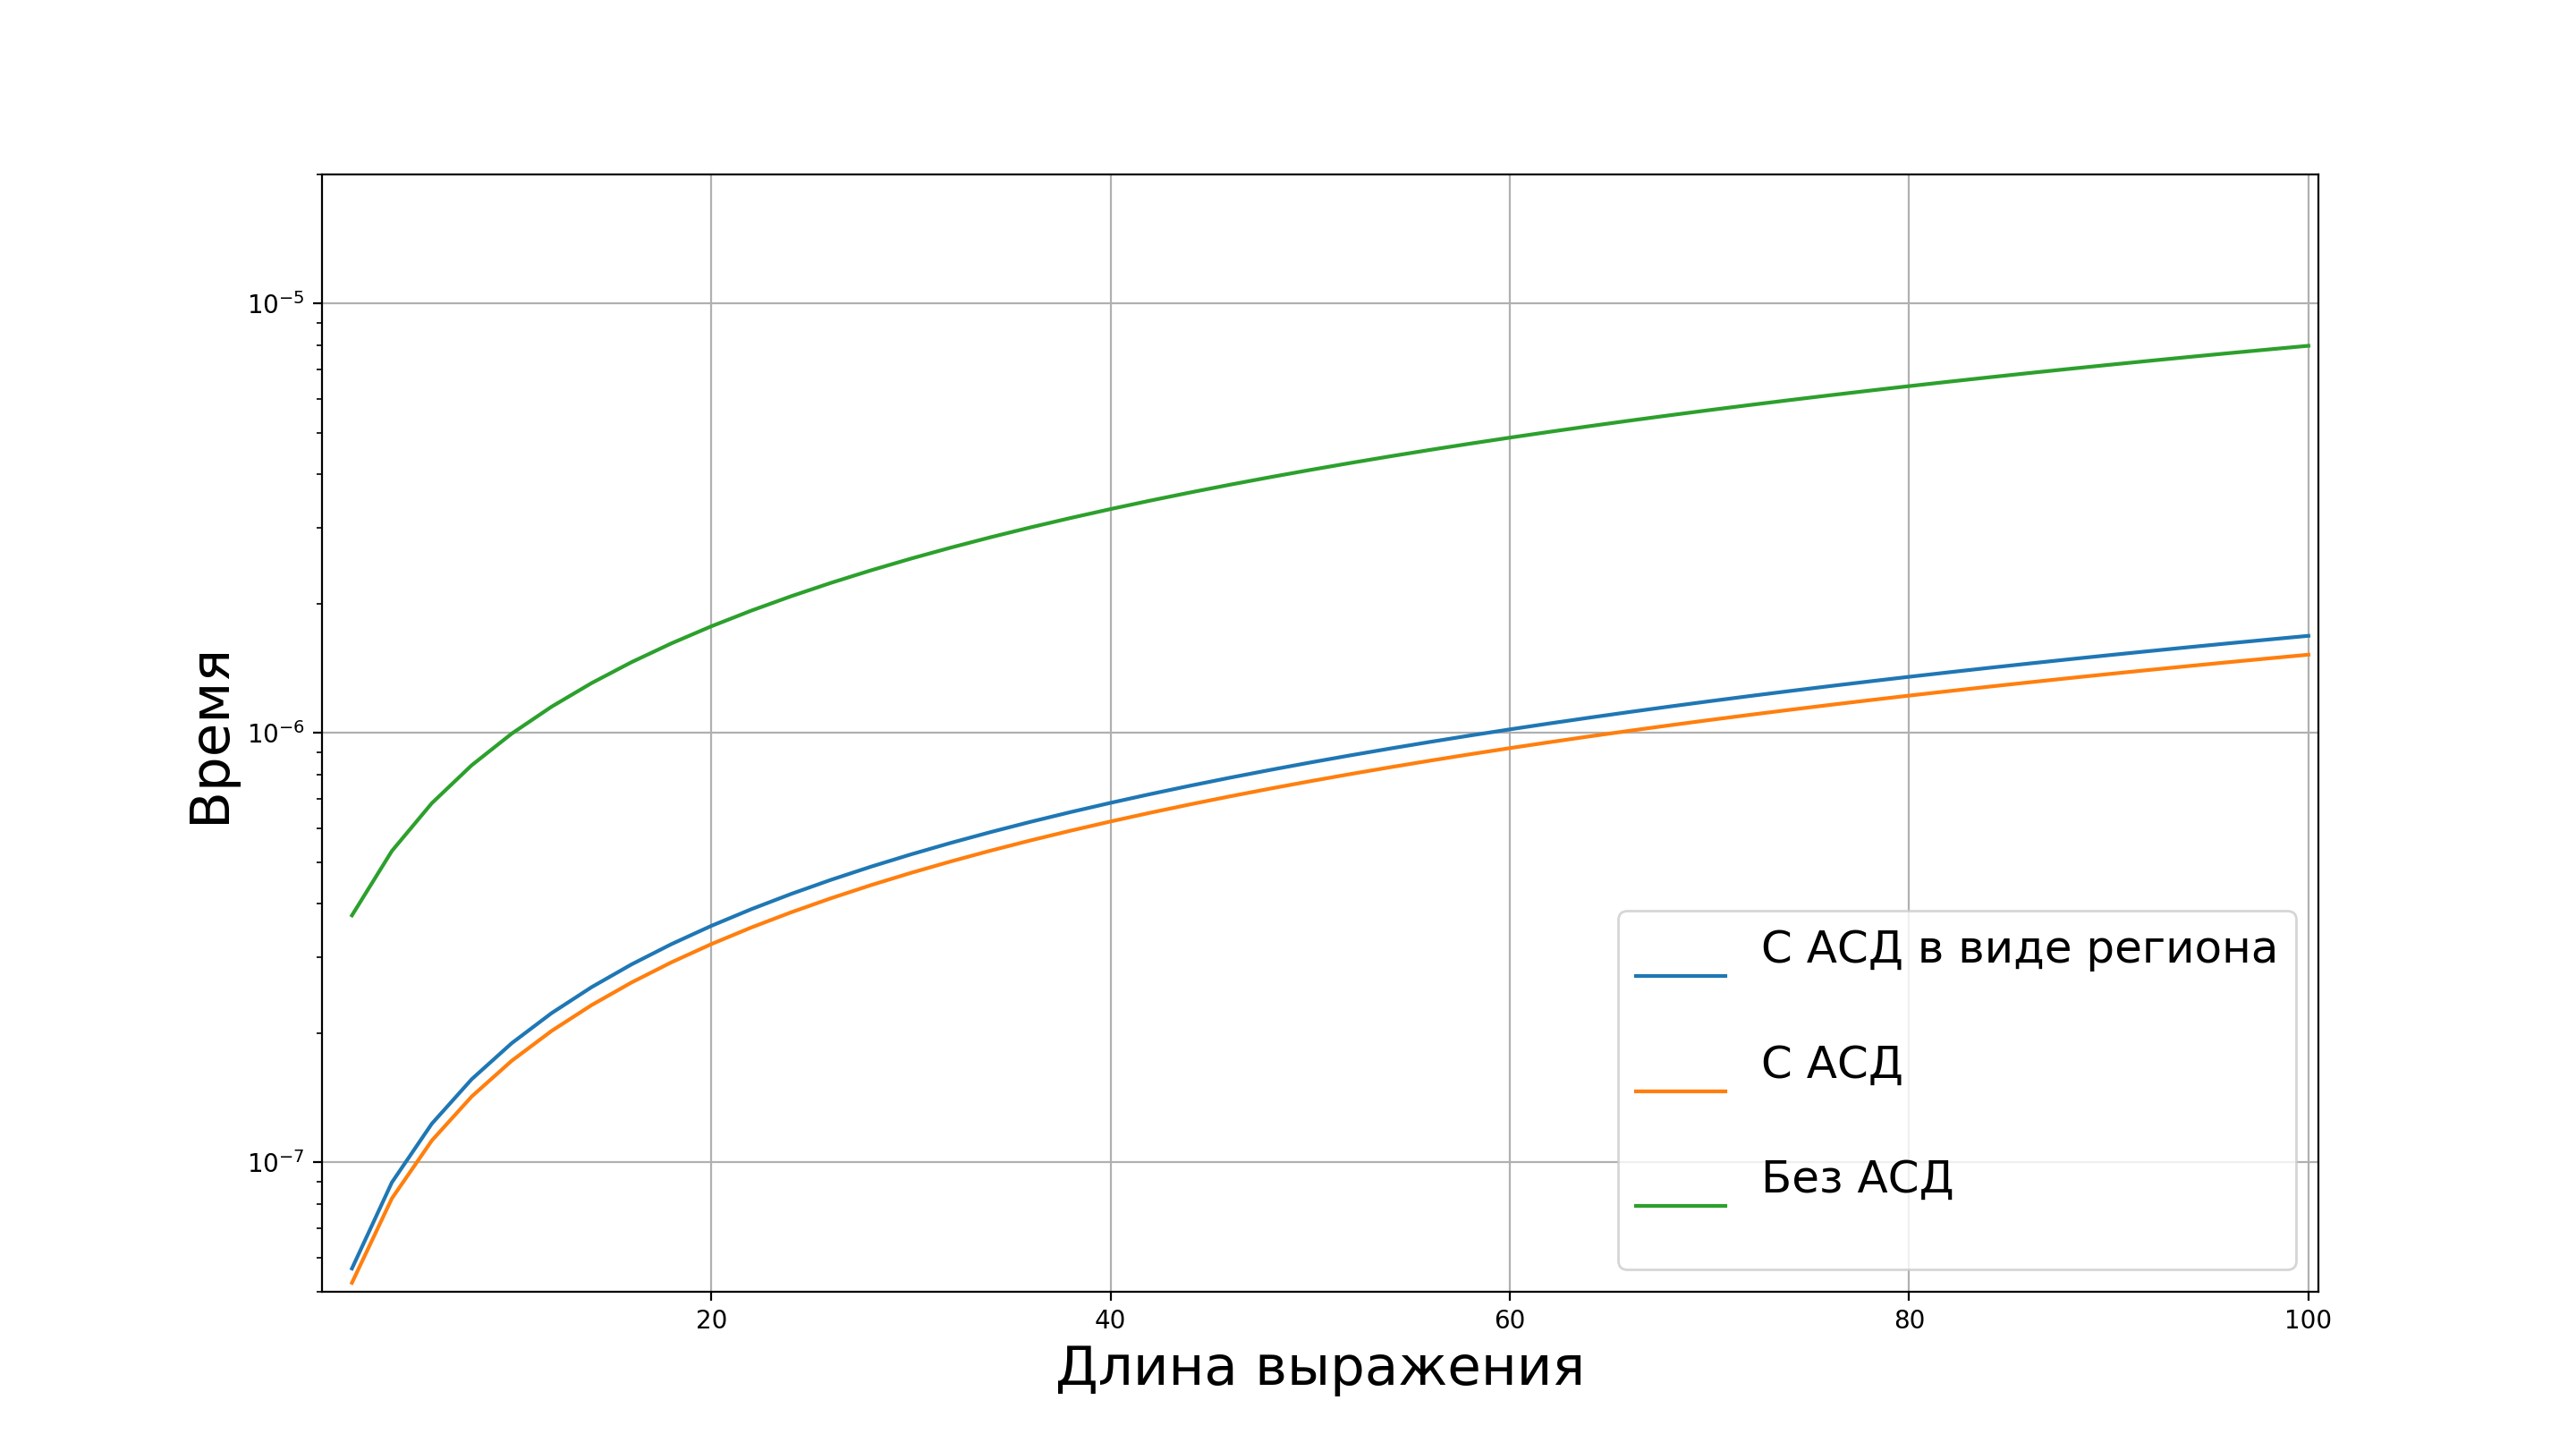
\includegraphics[scale=0.5]{benchmark.png}

\caption{Сравнение полученных результатов}

\label{fig:2}

\end{figure}
Исследование показало, что использование абстрактных синтаксических деревьев позволяет уменьшить время работы программы более чем в 5 раз, что существенно заметно для выражений любой длины.

Также из графиков видно, что в рамках данной работы не удалось добиться большей производительности при управлении памятью на основе регионов. Тем не менее, она все еще может считаться более предпочительной ввиду перечисленных ранее преимуществ.
\conclusion
В ходе данной работы:
\begin{enumerate}
    \itemБыли изучены теоретические основы построения лексических и синтаксических анализаторов.
    \itemПроанализированы особенности реализации лексических и синтаксических анализаторов.
    \itemБыли изучены принципы работы генераторов лексического и синтаксического анализа на примере Flex и GNU Bison.
    \itemБыли созданы лексический и синтаксический анализаторы для анализа математического выражения.
    \itemБыло изучено понятие абстрактного синтаксического дерева.
    \itemПроведен анализ производительности полученных реализаций.
\end{enumerate}

Таким образом, все поставленные в рамках работы задачи выполнены.

Результаты исследования показали, что абстрактные синтаксические деревья позволяют добиться увеличения производительности в 5–6 раз.

А это, в свою очередь, позволяет утверждать о том, что концепция абстрактных синтаксических деревьев является крайне важной в информатике и ее приложениях, в частности, при создании синтаксических анализаторов.
% Библиографический список, составленный вручную, без использования BibTeX
%
% \begin{thebibliography}{99}
%   \bibitem{Ione} Источник 1.
%   \bibitem{Itwo} Источник 2
% \end{thebibliography}

% Отобразить все источники. Даже те, на которые нет ссылок.
% \nocite{*}

% Меняем inputencoding на лету, чтобы работать с библиографией в кодировке
% `cp1251', в то время как остальной документ находится в кодировке `utf8'
% Credit: Никита Рыданов
%\inputencoding{cp1251}
\bibliographystyle{gost780uv}
\bibliography{thesis}
%\inputencoding{utf8}

% При использовании biblatex вместо bibtex
% \printbibliography

% Окончание основного документа и начало приложений Каждая последующая секция
% документа будет являться приложением
\appendix
\section{Flash-носитель с исходным кодом программ, использующихся в работе}
\label{app:А}
\noindent\textbf{Папка} \texttt{src} содержит оригинальный исходный код программы:

\textbf{Папка} \texttt{naive} "--- реализация без АСД

\textbf{Папка} \texttt{naiveast} "--- реализация с АСД

\textbf{Папка} \texttt{arena} "--- реализация с АСД на основе региона

\noindent\textbf{Папка} \texttt{extsrc} содержит измененный исходный код, необходимый для исследования производительности:

\textbf{Папка} \texttt{naive} "--- реализация без АСД

\textbf{Папка} \texttt{naiveast} "--- реализация с АСД

\textbf{Папка} \texttt{arena} "--- реализация с АСД на основе региона

\section{Исходный код программы на Python, осуществляющей исследование производительности полученных реализаций}
\label{app:Б}
\inputminted{python}{test.py}
\section{Исходный код программы на Python, осуществляющей анализ полученных результатов}
\label{app:В}
\inputminted{python}{graph.py}
\end{document}
